\newpage

\section{Detekcja oczu} \label{section:eye_detection}

W~tej pracy dyplomowej dużą role odgrywają oczy i~ich wpływ na sterowanie aplikacją. Z~tego powodu musiała zostać określona i~zaimplementowana skuteczna metoda ich detekcji.


\subsection{Algorytmy detekcji oczu}

Na potrzeby tego etapu zostały zastosowane dwie metody opierające się na algorytmach opisanych wcześniej - klasyfikatorach kaskadowych oraz znacznikach twarzy.


\subsubsection{Klasyfikator kaskadowy Haar}

Metody detekcji oparte na klasyfikatorach kaskadowych zostały opisane w rozdziale~\hyperref[{section:face_casacde_classifier}]{\ref{section:face_casacde_classifier}} przy okazji wykrywania twarzy. Do detekcji oczu z~użyciem tego algorytmu został wykorzystany model autorstwa Shameem Hameed \cite{eye_haar_model}.

\subsubsection{Znaczniki twarzy wokół oczu}

Opisane w rozdziale~\hyperref[section:landmarks]{\ref{section:landmarks}} algorytmy facemarków nanoszą punkty charakterystyczne na obraz twarzy. Znajdują się one m.in. wokół oczu. Fakt ten można wykorzystać do detekcji ich obszaru. Celem uzyskania takiego wyniku należy wyznaczyć prostokąt, który będzie otaczał wszystkie sześć znaczników danego oka. \cite{detect_eye_facemarks}

\par

Przykład takiego działania widoczny jest na rysunku~\ref{fig:facemarki_to_detect_eyes}.

\begin{figure}[!h]
    \begin{center}
        \subfigure[Znaczniki wokół oka]{\label{fig:facemarki_to_detect_eyes_no_rect}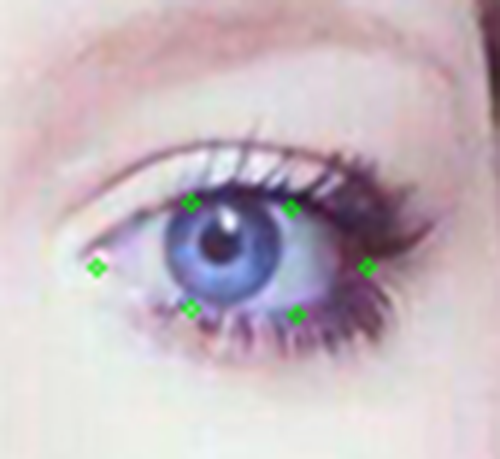
\includegraphics[scale=0.25]{img/eye_section/eye_facemarks.png}}
        \hspace{8mm}
        \subfigure[Naniesiony prostokąt otaczający znaczniki wokół oka]{\label{fig:facemarki_to_detect_eyes_rect}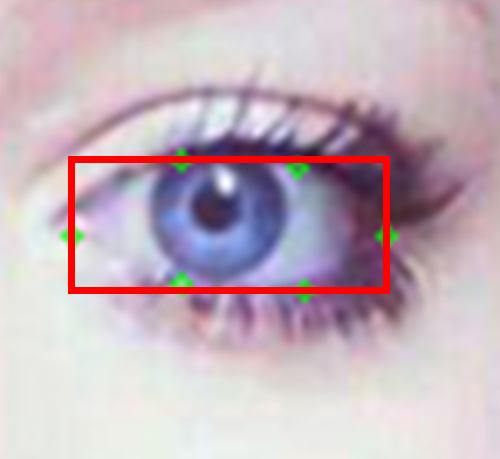
\includegraphics[scale=0.25]{img/eye_section/eye_facemarks_rect.png}}
    \end{center}
.    \caption{Wykorzystanie znaczników twarzy do detekcji obszaru oczu}
    \label{fig:facemarki_to_detect_eyes}
\end{figure}

Wykorzystywany jest tu też wskaźnik EAR (rozdz.~\hyperref[{section:EARsection}]{\ref{section:EARsection}}) do wykrycia czy oko jest zamknięte czy otwarte.

\par

Skuteczność detekcji oczu przy pomocy tej metody zależy w~dużym stopniu od dokładności algorytmu odwzorowującego punkty charakterystyczne twarzy. Ewentualne niedoskonałości można niwelować zwiększając wielkość prostokąta o~pewną tolerancję z~danej strony. Taki współczynnik w projekcie został testowo ustalony, a~przebieg badań i~wyników został opisany w rozdziale~\hyperref[{section:facemark_eye_size}]{\ref{section:facemark_eye_size}}.



\subsection{Filtrowanie wyników detekcji oczu metodą Haar}

Ze względu, że algorytm Haar może zwracać większą ilość prawdopodobnych obszarów, w~których spodziewa się on wykryć pożądany obiekt, wprowadzone zostało filtrowanie wyników detekcji oczu. 

\par

Algorytm filtrowania składa się z dwóch etapów:

\begin{itemize}
    \item Podzielenie wykrytych obszarów na dwie grupy - na lewą i~prawą stronę twarzy
    \item W obu grupach wybranie największego obszaru
\end{itemize}


Dodatkowo pozwoliło to na łatwe zidentyfikowanie który obszar to które oko i~ich posortowanie.

\par

Przykładowy rezultat takiego filtrowania pokazany jest na \hyperref[{fig:eye_filter}]{rysunku~\ref{fig:eye_filter}}. 


\begin{figure}[!h]
    \begin{center}
        \subfigure[Przed filtrowaniem]{\label{fig:eye_filter_before}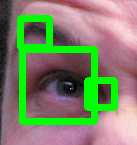
\includegraphics[scale=1.0]{img/eye_section/eye_filter_before.png}}
        \hspace{8mm}
        \subfigure[Po filtrowaniu]{\label{fig:eye_filter_after}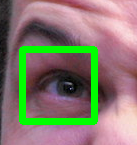
\includegraphics[scale=1.0]{img/eye_section/eye_filter_after.png}}
    \end{center}
    \caption{Efekt filtrowania obszarów detekcji oczu metodą klasyfikatorów kaskadowych Haar.}
    \label{fig:eye_filter}
\end{figure}

\subsection{Obcięcie obszaru twarzy dla detekcji oczu metodą Haar}

Dla metody opartej na Haar zdecydowano się dodatkowo zawęzić płaszczyznę przeszukiwań o~pewną część twarz, celem uzyskania wyników lepszych niż bez takiego zmniejszenia. 

\par

Ustalenie jaki obszar da najlepszy rezultat odbyło się przez testowe sprawdzanie kombinacji trzech parametrów oznaczających jaka część wykrytej twarzy zostaje obcięta z~poszczególnych stron. Mogły one przyjmować wartości w~następujących przedziałach:

\begin{itemize}
    \item Góra: $[0.0,$ $0.2]$
    \item Dół: $[0.2,$ $0.6]$
    \item Boki: $[0.0,$ $0.2]$
\end{itemize}

Każdy parametr przyjmował kolejne wartości będące wielokrotnością $0.05$ w~poszczególnych przedziałach.

\par

Ze względu na dużą ilość kombinacji ($225$) nie zostały podane wyniki, a~jedynie najlepsza kombinacja:

\begin{itemize}
    \item Góra: $0.05$
    \item Dół: $0.3$
    \item Boki: $0.0$
\end{itemize}

Algorytm Haar uzyskał lepszą skuteczność detekcji wykorzystując dodatkowe obcięcie niż bez niego - tabela~\ref{tab:eye_haar_crop_result}.

\begin{table}[!h]

\centering
\caption{Skuteczność algorytmu detekcji oczu Haar z dodatkowym obcięciem i bez}
\label{tab:eye_haar_crop_result}
\resizebox{\textwidth}{!}{%
\begin{tabular}{|c|c|c|c|c|c|c|}
\hline
 &
  \textbf{\begin{tabular}[c]{@{}c@{}}Prawidłowe\\ detekcje\end{tabular}} &
  \textbf{\begin{tabular}[c]{@{}c@{}}Perfekcyjne\\ detekcje\end{tabular}} &
  \textbf{\begin{tabular}[c]{@{}c@{}}Częściowo\\ dobre\\ detekcje\end{tabular}} &
  \textbf{\begin{tabular}[c]{@{}c@{}}Złe\\ detekcje\end{tabular}} &
  \textbf{\begin{tabular}[c]{@{}c@{}}Niewykryte\\  oczy otwarte\end{tabular}}  &
 \textbf{\begin{tabular}[c]{@{}c@{}}Niewykryte\\  oczy zamknięte \end{tabular}} \\ \hline \hline
\textbf{Haar bez obcięcia} &
  124 &
  85 &
  39 &
  34 &
  8 &
  32  \\ \hline

\textbf{Haar z obcięciem} &
  133 &
  95 &
  38 &
  23 &
  9 &
  11  \\ \hline
  
  \hline
\end{tabular}%
}
\end{table}

Przykład takiego obcięcia z wybranymi parametrami widoczny jest na \hyperref[{fig:eye_crop}]{rysunku~\ref{fig:eye_crop}}.

\begin{figure}[!h]
    \begin{center}
        \subfigure[Wykryty obszar twarzy]{\label{fig:eye_crop_before}
\includegraphics[scale=0.6]{img/eye_section/eye_cropped_face.png}}
        \hspace{8mm}
        \subfigure[Obszar po obcięciu]{\label{fig:eye_crop_after}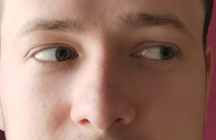
\includegraphics[scale=0.6]{img/eye_section/eye_cropped_eyes.png}}
    \end{center}
    \caption{Obcięcie obszaru detekcji oczu zgodnie z dobranymi wcześniej parametrami.}
    \label{fig:eye_crop}
\end{figure}

Wprowadzenie takiej modyfikacji pozwoliło odrzucić część błędnie ustalanych obszarów, szczególnie w dolnej części twarzy. Przykład poprawionej detekcji oczu dzięki temu zabiegowi widoczny jest na rysunku \ref{fig:eye_detect_crop}

\begin{figure}[!h]
    \begin{center}
        \subfigure[Wykrywanie oczu bez dodatkowego obcięcia obszaru]{\label{fig:eye_detect_crop_before}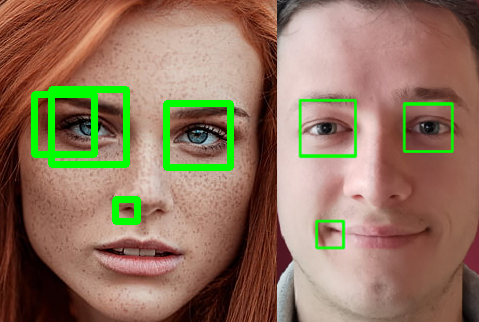
\includegraphics[scale=0.45]{img/eye_section/eye_detect_before_crop_1.png}}
        \hspace{8mm}
        \subfigure[Wykrywanie oczu z dodatkowym obcięciem obszaru]{\label{fig:eye_detect_crop_after}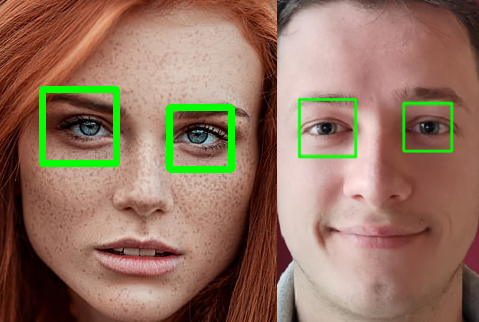
\includegraphics[scale=0.45]{img/eye_section/eye_detect_after_crop_1.png}}
    \end{center}
    \caption{Odrzucenie błędnych rezultatów detekcji oczu metodą Haar po dodatkowym obcięciu obszaru. Źródło pierwszego zdj.:\cite{readheadPortrait2}}
    \label{fig:eye_detect_crop}
\end{figure}


\subsection{Dostosowanie rozmiaru zwracanego obszaru oczu dla znaczników twarzy} \label{section:facemark_eye_size}

Dla metody opartej o punkty charakterystyczne twarzy zdecydowano się dodać pewną tolerancję do obszaru oczu wynikającego jedynie z~połączenia tych punktów.

\par

Ustalenie jakie zwiększenie zwracanego regionu da najlepsze rezultaty detekcji oczu odbyło się przez testowe sprawdzenie kombinacji trzech parametrów, które oznaczały wielkość tolerancji z~danej strony. W trakcie testu przyjmowały one następujące wartości:

\begin{itemize}
    \item Góra: z przedziału [0.0, 1.0], będące wielokrotnością $0.1$
    \item Dół: z przedziału [0.0, 1.0], będące wielokrotnością $0.1$
    \item Boki: z przedziału [0.0, 0.5], będące wielokrotnością $0.05$
\end{itemize}

\par

Ze względu na dużą ilość kombinacji ($1331$) nie zostały podane wyniki, a~jedynie wybrana najlepsza kombinacja:

\begin{itemize}
    \item Góra: $0.7$
    \item Dół: $0.5$
    \item Boki: $0.2$
\end{itemize}


\begin{table}[!h]
\label{tab:eye_facemark_size_result}
\centering
\caption{Skuteczność algorytmu detekcji oczu wykorzystując facemarki z dodatkowym zwiększeniem obszaru i bez}
\resizebox{\textwidth}{!}{%
\begin{tabular}{|c|c|c|c|c|c|c|}
\hline
 &
  \textbf{\begin{tabular}[c]{@{}c@{}}Prawidłowe\\ detekcje\end{tabular}} &
  \textbf{\begin{tabular}[c]{@{}c@{}}Perfekcyjne\\ detekcje\end{tabular}} &
  \textbf{\begin{tabular}[c]{@{}c@{}}Częściowo\\ dobre\\ detekcje\end{tabular}} &
  \textbf{\begin{tabular}[c]{@{}c@{}}Złe\\ detekcje\end{tabular}} &
  \textbf{\begin{tabular}[c]{@{}c@{}}Niewykryte\\  oczy otwarte\end{tabular}}  &
 \textbf{\begin{tabular}[c]{@{}c@{}}Niewykryte\\  oczy zamknięte \end{tabular}} \\ \hline \hline
\textbf{\begin{tabular}[c]{@{}c@{}}Facemarki oczu \\ bez zwiększenia obszaru\end{tabular}} &
  142 &
  17 &
  125 &
  14 &
  6 &
  6  \\ \hline

\textbf{\begin{tabular}[c]{@{}c@{}}Facemarki oczu \\ ze zwiększeniem obszaru\end{tabular}} &
  144 &
  142 &
  2 &
  12 &
  6 &
  6  \\ \hline
  
  \hline
\end{tabular}%
}
\end{table}

Zmiana wielkości zwracanego obszaru oczu nie zwiększył znacząco liczby dobrych detekcji. Natomiast największy zysk widoczny jest w~perfekcyjnych detekcjach. Dzięki takiemu dostosowaniu udało się osiągnąć prawie $100\%$ wskaźnik perfekcyjnych względem prawidłowych detekcji. Pozwoli to uzyskać lepiej dobraną wielkość obszaru oczu, co może mieć przełożenie na skuteczność detekcji źrenic.